\documentclass{article}

\usepackage[margin=2.5cm,left=2cm,includefoot]{geometry}
\usepackage{graphicx}
\usepackage{float}
\usepackage[space]{grffile}
\usepackage{hyperref}
\usepackage[export]{adjustbox}
\usepackage{multicol}
\usepackage{caption}
\usepackage{hyperref}
\usepackage{listings}
\usepackage{vhistory}
\usepackage{titlesec}

\setcounter{secnumdepth}{4}

\titleformat{\paragraph}
{\normalfont\normalsize\bfseries}{\theparagraph}{1em}{}
\titlespacing*{\paragraph}
{0pt}{3.25ex plus 1ex minus .2ex}{1.5ex plus .2ex}

% Header and footer
\usepackage{fancyhdr}
\pagestyle{fancy}

\rhead{COS301}
\lhead{User Manual Document}
\fancyfoot[R]{Page \thepage}

\renewcommand{\headrulewidth}{2pt}
\renewcommand{\footrulewidth}{1pt}

\begin{document}

	\begin{titlepage}
		\begin{center}
			
\includegraphics[width=10cm]{images/logo.png}  \\
			[0.5cm]
			\huge{
			User Manual Document\\
			}
			
			\line(1,0){300}\\
			[0.2cm]
			\LARGE{Project: MarketLead.io\\
			Client: RetroRabbit} \\
			\line(1,0){300}\\
			\LARGE{Team: Valknut Solutions}\\
			[1.0cm]
			\large{Version: 1.1}\\
			[1.0cm]
			\large
			{
			\begin{itemize}
				\item 13054903 - Charl Jansen van Vuuren    
				\item 13044924 - Kevin David Heritage
				\item 13176545 - Quinton Weenink\\
			\end{itemize}
			}
			\textsc{\large}\\
		[3.0cm]
		\textsc{\large  Department of Computer Science}\\
		[0.5cm]
		\textsc{\large \today}\\
		\end{center}
	\end{titlepage}
	
	\cleardoublepage
	% Start of the revision history table
	\begin{versionhistory}
  		\vhEntry{1.0}{27.7.2016}{CJvV,KH,QW}{in progress}
  		\vhEntry{1.1}{9.9.2016}{CJvV,KH,QW}{Changed product name. Update manual structure. Updates for new use cases and modules.}
  		\vhEntry{1.2}{11.10.2016}{CJvV,KH,QW}{Updated according to feedback. Added new functionality manual. Updated the logo}
	\end{versionhistory}	
	
	\cleardoublepage
	\tableofcontents
	\cleardoublepage
	
	\section{General Information}
		\subsection{System Overview}
			%Too vague for an outsider
			%State what kind of info is gathered and who may have an interest in this information and what benifits they can gain from having the info
			%Briefly state what the system provides to assist the interested party in using the gathered information.
			%Language and spelling error checks
			MarketLead.io is a real time marketing and lead gathering application with multiple integration points with social media and other formats.\\
			A business can manage and respond to leads and analyze their current customers and we expose and link companies to their future customers in an easy and pluggable manner.

			This document contains information related to the use of the MarketLead.io system and how to use it.
			The purpose of the system is to gather information from various social media platforms (i.e. from Facebook Messenger, Facebook Lead Ads, We Chat). The data that was gathered can then be visualized in different graphs for analysts. 
			Users that are interested in a product that the system has to offer does not necessarily work with the system directly but rather through the various social media platforms.
			A marketer can register their different social media platforms to interact with the system through the website.
			This user manual provides information on how to interact with the web interface for administrators, analysts and marketers. 
			Working through this user manual can give anyone interacting with the web interface moor information on how to use the system efficiently and correctly.
			This user manual is not for the clients/users on the social media platforms rather for the analysts and marketers that physically interact with the system.

		\subsection{System Configuration} %TODO: Create the image of the system or something
			%extended to mention the info resources that are connected. 
			%Image of web server connected to different source to provide info and some client machines connected to the server
			The main input of data to the system will be from the various social media platforms from clients. Marketers and analysts will use the web interface to use the system.
			
		\subsection{Installation}%Refer user to browser settings on chrome and firefox web sites to activate the necesarry settings for their browser to work correctly with our system0
			The system does not have to be installed how ever an up to date web browser is required to view the web site that interacts with the system. Mozilla Firefox or Google Chrome is recommended.

	\section{Getting Started}
		A user/client needs to be signed up for the various social media platforms that the system uses.
		Marketers should also have accounts at the various social media platforms.
		Analysts will receive a login from an administrator of the system to be able to log into the system and see analytics.\\
		Marketers and analysts can open their web browser (Mozilla Firefox/Chrome recommended) and go to \href{https://insuranceprofiling.herokuapp.com}{MarketLead.io} to get started with their various tasks.
		When the marketer/analyst is done using the system they can simply close the web browser window to end their session with the system.

	\section{Using the system}
		In order to use the system you will have to navigate to the website.
		Open a web browser of your choice (Mozilla Firefox/Google Chrome recommended) and navigate to the \href{https://insuranceprofiling.herokuapp.com}{MarketLead.io} website.
		\subsection{Signing up your page}
			This section will cover the steps necessary for signing up your Facebook page in order for Facebook to send the data from the Lead Ads on your page through to the MarketLead.io server for processing.
			\begin{enumerate}
				\item Navigate to the website\\
				Open up the browser of your choice (Mozilla Firefox recommended) and navigate to the \href{https://insuranceprofiling.herokuapp.com}{Insurance Profiling} website.

				\item Sign up\\
				Click on the Sign Up button in the top right corner of the website\\
				\begin{figure}[H]
				  \centering
				      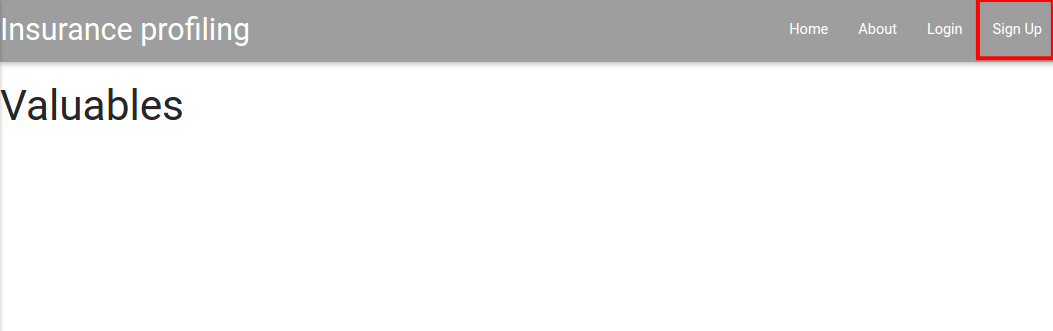
\includegraphics[width=\textwidth]{images/home_signup.png}
				  \caption{Home page indicating where to sign up}
				  \label{fig:homeSignup}
				\end{figure}

				\item Login with Facebook\\
				Once redirected click the button to Login with Facebook\\
				\begin{figure}[H]
				  \centering
				      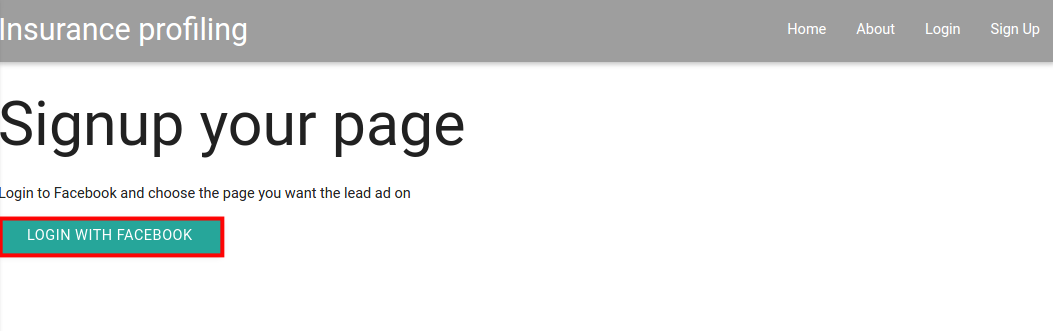
\includegraphics[width=\textwidth]{images/signup_login.png}
				  \caption{Button to click to login with Facebook}
				  \label{fig:signupLogin}
				\end{figure}
				When you have clicked the button a pop-up will appear requesting you to log into Facebook requesting permissions for the system to manage your pages.

			\item Selecting the page to manage\\
				Once the user has logged into their Facebook account with permission to manage their pages, a list of their pages will be displayed.\\
				Select the page that the system needs to manage.\\
				\begin{figure}[H]
				  \centering
				      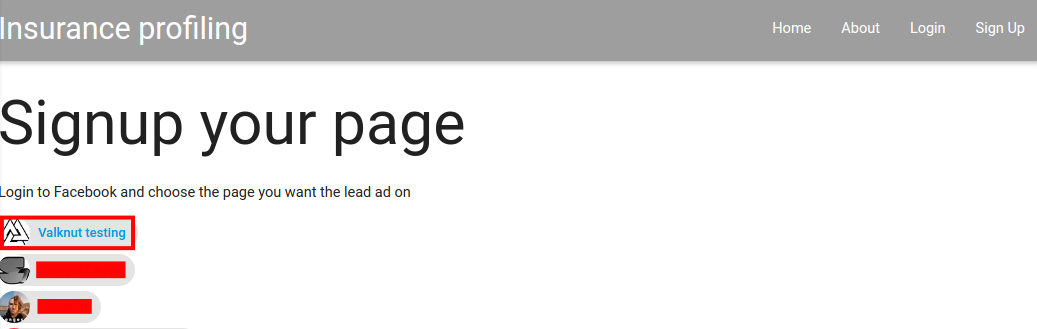
\includegraphics[width=\textwidth]{images/select_page.png}
				  \caption{Selecting the page to manage}
				  \label{fig:selectPage}
				\end{figure}
				When clicking on the page that the system should manage a pop-up will appear that requires the user to accept the Facebook lead ads terms of service. The system cannot manage the lead ad without the marketer of the page accepting their terms of service.\\
				\begin{figure}[H]
					\centering
						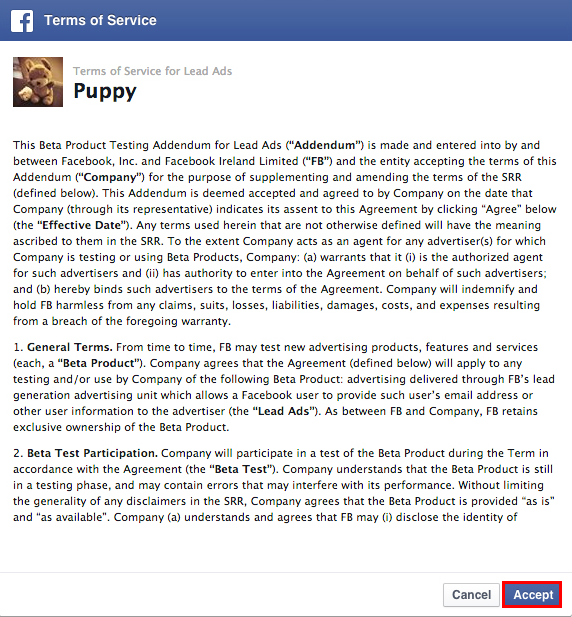
\includegraphics[width=\textwidth]{images/facebook_tos.png}
					\caption{Facebook terms of service}
					\label{fig:facebookTermsOfService}
				\end{figure}
				Once the terms of service has been accepted a lead ad can be created through the form creator.\\
				\begin{figure}[H]
					\centering
						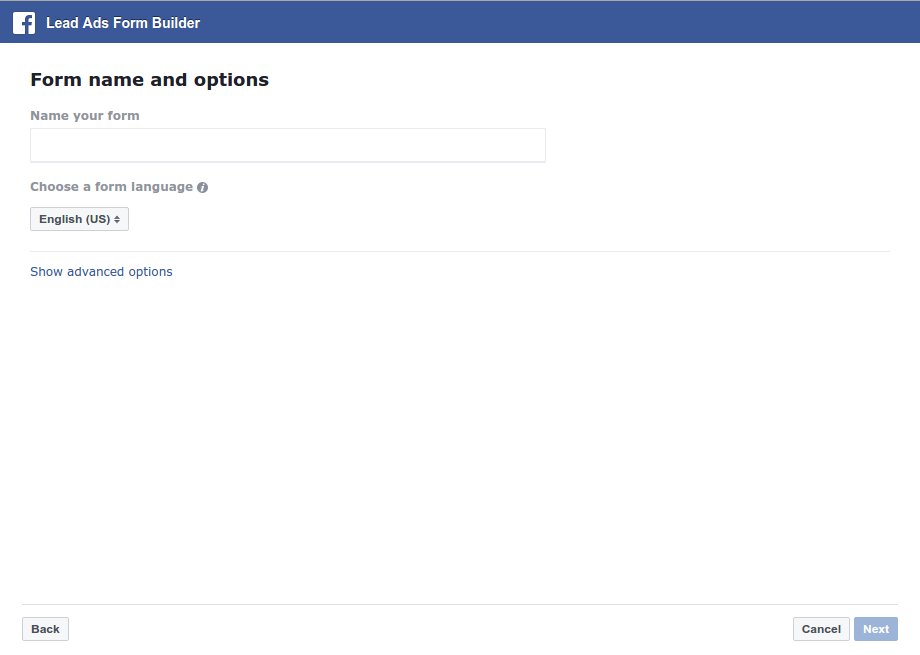
\includegraphics[width=\textwidth]{images/facebook_lead_form_creator.png}
					\caption{Facebook lead form creator}
					\label{fig:facebookLeadFormCreator}
				\end{figure}
				*Incomplete: Process being implemented (Server still accepts lead data from lead ads created through the following reference*\\
				To create a lead ad use this Facebook references: \href{https://www.facebook.com/business/a/lead-ads}{Facebook Lead adverts}
			\end{enumerate}

		% \subsection{Manually filling in a lead}
		% 	If a user wants to use a service and does not use the various social media platforms they can navigate to the \href{https://insuranceprofiling.herokuapp.com}{MarketLead.io} and fill in a lead form manually.
		% 	\begin{enumerate}
		% 		\item 
		% 	\end{enumerate}

		\subsection{Generating reports}
			\begin{enumerate}
				\item Navigate to the 'Reports' page
					\begin{figure}[H]
						\centering
							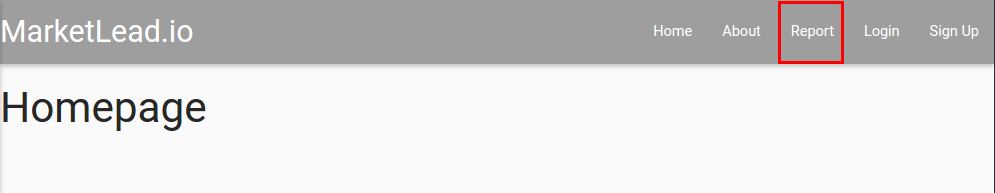
\includegraphics[width=\textwidth]{images/home_reports.png}
						\caption{Home page indicating where to find reports}
						\label{fig:homeReports}
					\end{figure}
					After this has been clicked the page will load the report generator.
				\item Create a report
					\begin{figure}[H]
						\centering
							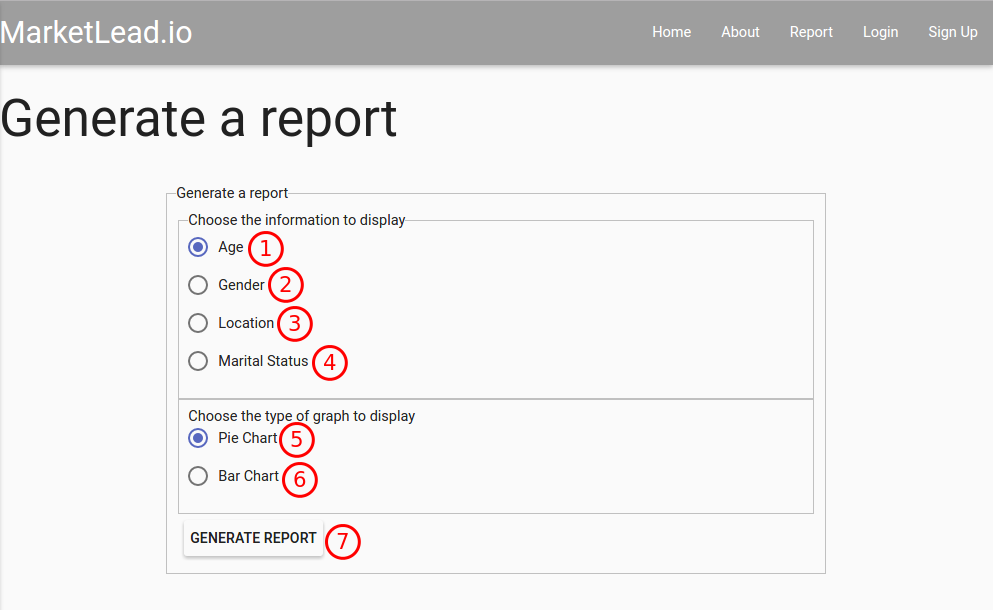
\includegraphics[width=\textwidth]{images/generate_report.png}
						\caption{Report generator}
						\label{fig:reportGenerator}
					\end{figure}
					Breakdown of the report generator
					\begin{itemize}
						\item[1.] When selecting this item there will be a graph of the amount of clients falling different age groups.
						\item[2.] When selecting this item there will be a graph of the amount of clients falling in the different genders
						\item[3.] When selecting this item there will be a graph of the amount of clients in the different locations
						\item[4.] When selecting this item there will be a graph of the amount of clients in different marital statuses
						\item[5.] This item will produce a Pie Chart graph
						\item[6.] This item will produce a Bar Chart graph
						\item[7.] This button will generate a report according to the options selected above and it will be displayed below the graph generator.
					\end{itemize}
			\end{enumerate}
	
	\section{Troubleshooting}
		\begin{itemize}
			\item When the website does not load: check your Internet connection and then refresh the page.
			\item When the 'Login with Facebook' button does not show up for a period of time (30 seconds) try refreshing the web page by pressing 'F5' on your keyboard or clicking the refresh button in your browser.
			\item When nothing shows up after generating a report there may be no data to generate a report from and a blank graph will be displayed with no data.
		\end{itemize}

	\section{References to other documentation}
		\begin{itemize}
			\item{Requirements specifications as per 11 September 2016}
			\item{Architecture Design as per 11 September 2016}
			\item{\href{https://www.facebook.com/business/a/lead-ads}{Facebook Lead adverts} as per 29 July 2016}
		\end{itemize}

	\section{Signing up your page}
		This section will cover the steps necessary for signing up your Facebook page in order for Facebook to send the data from the Lead Ads on your page through to the Insurance profiling server for processing.
		\begin{enumerate}
			\item Navigate to the website\\
			Open up the browser of your choice (Mozilla Firefox recommended) and navigate to the \href{https://insuranceprofiling.herokuapp.com}{Insurance Profiling} website.

			\item Sign up\\
			Click on the Sign Up button in the top right corner of the website\\
			\begin{figure}[H]
			  \centering
			      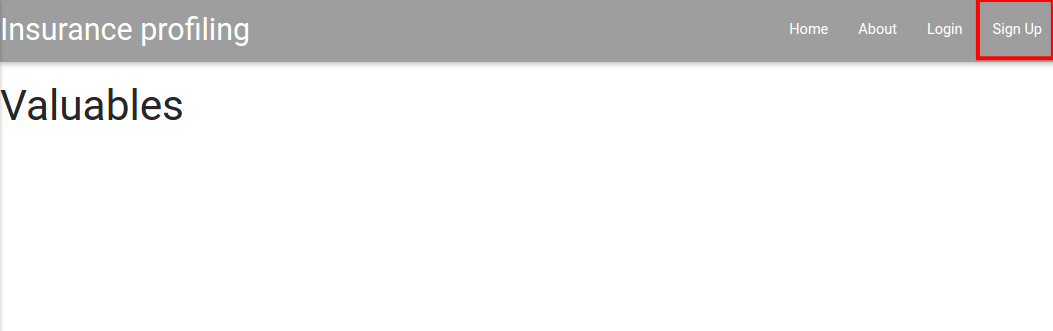
\includegraphics[width=\textwidth]{images/home_signup.png}
			  \caption{Home page indicating where to sign up}
			  \label{fig:homeSignup}
			\end{figure}

			\item Login with Facebook\\
			Once redirected click the button to Login with Facebook\\
			\begin{figure}[H]
			  \centering
			      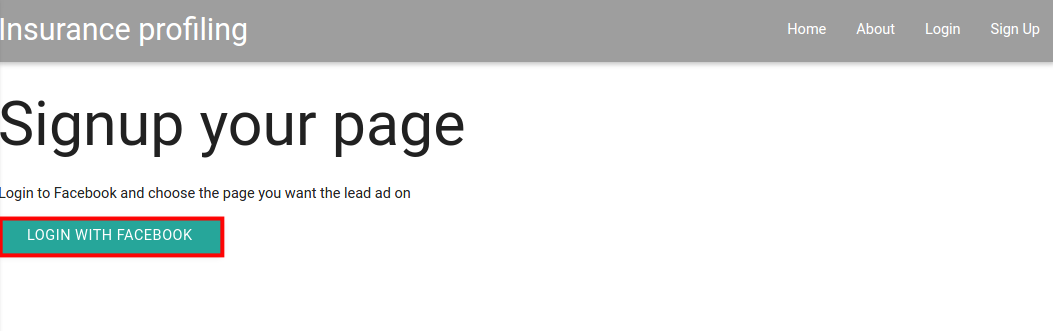
\includegraphics[width=\textwidth]{images/signup_login.png}
			  \caption{Button to click to login with Facebook}
			  \label{fig:signupLogin}
			\end{figure}
			When you have clicked the button a pop-up will appear requesting you to log into Facebook requesting permissions for the system to manage your pages.

		\item Selecting the page to manage\\
			Once the user has logged into their Facebook account with permission to manage their pages, a list of their pages will be displayed.\\
			Select the page that the system needs to manage.\\
			\begin{figure}[H]
			  \centering
			      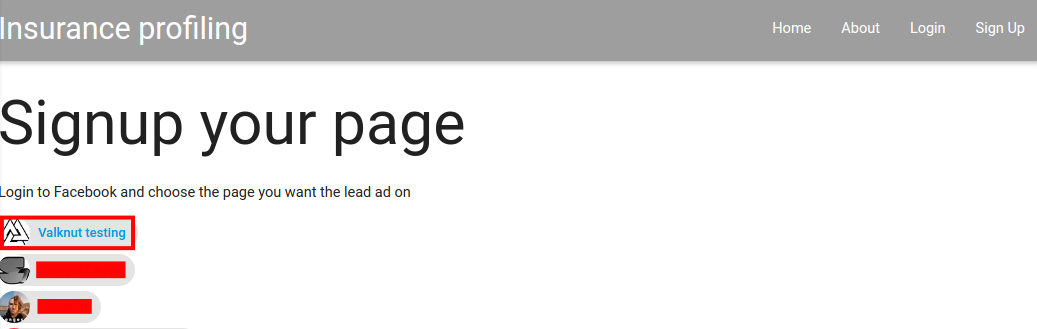
\includegraphics[width=\textwidth]{images/select_page.png}
			  \caption{Selecting the page to manage}
			  \label{fig:selectPage}
			\end{figure}
			When clicking on the page that the system should manage the user can create a lead ad.\\
			To create a lead ad user this Facebook references: \href{https://www.facebook.com/business/a/lead-ads}{Facebook Lead adverts}
		\end{enumerate}

\end{document}
